\documentclass[12pt]{article}
\usepackage[left=1in, right=1in, top=1in, bottom=1in]{geometry}
\usepackage{amsmath}
\newcommand{\N}{\mathbb{N}}
\newtheorem{theorem}{Theorem}[section]
\newtheorem{lemma}[theorem]{Lemma}
\newtheorem{claim}[theorem]{claim}
\newtheorem{prop}{Proposition}
\usepackage{tikz}
\usetikzlibrary{automata,positioning,arrows}
\usepackage{algorithm}
\usepackage{algpseudocode}
\usepackage{enumitem}
\begin{document}
\begin{center}
\section*{$\sim$ Assignment 3  Computational Models Spring 2022 $\sim$}
\subsubsection*{Saar Barak}
\end{center}
\subsection*{Exercise 1}
Considering the following language\[
\mathcal{L=} \{ \# 1^n \# x_1  \ldots x^n : \exists i\neq j \text{ s.t }
x_i \neq x_j \}
\]
Lets describe an 2-tape NTM $\mathcal{M}$ that allow the head  to stay at the same place, that recive input $\# 1^n \# (n > 1)$ and  implements the first part of decide $\mathcal{L}$
\[
Q=\lbrace q_0,q_a,q_r \rbrace,\Sigma =\{ 1,\# \},\Gamma =\{ 1,\# ,\sqcup \} 
\]
and define $\delta$ :

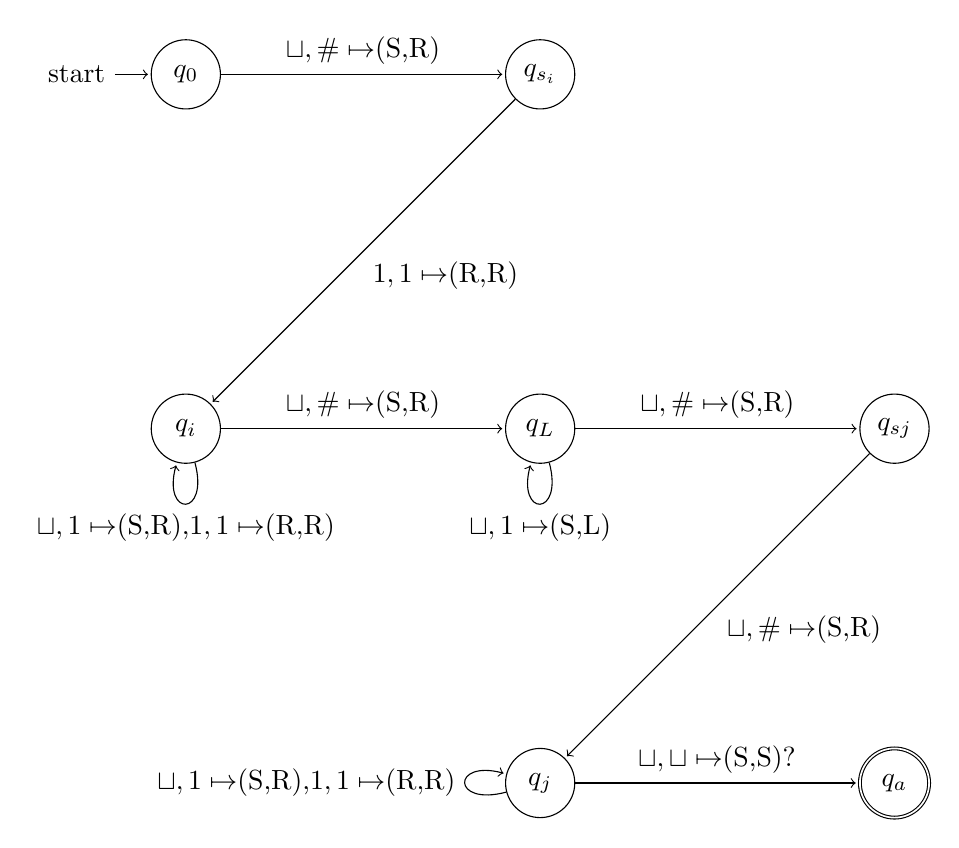
\begin{tikzpicture}[shorten >=1pt,node distance=4.5cm,on grid,auto] 
   \node[state,initial] (q_0)   {$q_0$}; 
   \node[state] (q_1) [ right=of q_0] {$q_{s_i}$}; 
   \node[state] (q_3) [below =of q_0] {$q_i$};
   \node[state] (q_4) [below  =of q_1] {$q_{L}$};     
   \node[state] (q_6) [right  =of q_4] {$q_{sj}$};        
   \node[state] (q_5) [below  =of q_4] {$q_j$};
   \node[state,accepting] (q_a) [below  =of q_6] {$q_a$};

    \path[->] 
    (q_0) edge  node {$\sqcup,\# \mapsto$(S,R)} (q_1)
    (q_1) edge node  {$1,1 \mapsto$(R,R)} (q_3)
    (q_3) edge  node {$\sqcup,\# \mapsto$(S,R)} (q_4)
    edge[loop below] node{$\sqcup,1 \mapsto$(S,R),$1,1 \mapsto$(R,R)}()
    (q_4) edge  node {$\sqcup,\# \mapsto$(S,R)} (q_6)
     edge[loop below] node{$\sqcup,1 \mapsto$(S,L)}()
    (q_6) edge  node {$\sqcup,\# \mapsto$(S,R)} (q_5)
     (q_5) edge[loop left] node{$\sqcup,1 \mapsto$(S,R),$1,1 \mapsto$(R,R)}()
     edge  node {$\sqcup,\sqcup \mapsto$(S,S)?} (q_a)
;
\end{tikzpicture}
\\The idea behind the way I generated $\delta$ is first to verify we start "legal" sequence i.e $i \neq j$ and $ i,j >0$ and split  non-deterministic for any  $i,j$ the NTM run
\pagebreak
\subsection*{Exercise 2}
\subsubsection*{(a)}For DFA  $A = (Q, \Sigma, \delta, q_0, F)$. lets describe a 2-tape TM M that accept $\mathcal{L}(A)$
\[
Q=\lbrace q_{m},q_a,q_r \rbrace,\Sigma =\Sigma ,\Gamma =\Sigma \cup\{\{q\in Q\} ,\sqcup \},q_0=q_{m}
\]
\[ \delta(q,(\sigma_1,\sigma_2))=
\begin{cases} 
      (q_m,(\sigma_1,\delta(q_0,\sigma_1),(R,L)) &\quad\text{if  } \sigma_1 \in \Sigma \wedge\sigma_2=\sqcup\\
       (q_m,(\sigma_1,\delta(\sigma_1,\sigma_2)),(R,L)) &\quad\text{if } \sigma_1 \in \Sigma \wedge\sigma_2=q\in Q/F \\
       (q_a,(\sigma_1,\sigma_2),(R,L)) &\quad\text{if } \sigma_1= \sqcup \wedge\sigma_2=q\in F \\
       (q_r,(\sigma_1,\sigma_2),(R,L)) &\quad\text{if } \sigma_1= \sqcup \wedge\sigma_2=q\notin F \\
     \end{cases}  
     \]   
The idea is to save the last visted state on of A.
\subsubsection*{(b)}
For TM  $M = (Q, \Sigma, \delta, q_0, F)$. lets describe a 2-tape TM $M_2$ that accept $\mathcal{L}(M)$
\[
Q=\lbrace q_{m2},q_a,q_r \rbrace,\Sigma =\Sigma ,\Gamma =\Sigma \cup\{q\in Q\} ,q_0=q_{m2}
\]
Lets define  $\hat{q},\hat{\sigma},\hat{D}$ to be the triplet such that $\delta(q,\sigma)\longmapsto (\hat{q},\hat{\sigma},\hat{D})$
\[ \delta(q,(\sigma_1,\sigma_2))=
\begin{cases} 
      (q_m,(\hat{\sigma},\hat{q}),(\hat{D},L)) &\quad\text{if  } \sigma_1 \in \Sigma \wedge\sigma_2=\sqcup\\
       (q_m,(\hat{\sigma},\hat{q}),(\hat{D},L)) &\quad\text{if } \sigma_1 \in \Sigma \wedge\sigma_2=q\in Q \\
       (q_a,(\sigma_1,q_a),(R,L)) &\quad\text{if }  \sigma_2=q_a \wedge \forall \sigma_1 \\
       (q_r,(\sigma_1,q_r),(R,L)) &\quad\text{if }\sigma_2=q_r \wedge \forall \sigma_1 \\ \end{cases}  
     \]  The idea is kind of same as above but now we track the direction of the head of M 
     \pagebreak
\subsection*{Exercise 3}
\begin{prop} Disprove $\mathcal{RE}$ is not closed under complement.\end{prop}
For $L,\overline{L}$, if both are semi-decidable $\Rightarrow$ both are decidable, (can just flip the nation reject accept)
$\Rightarrow$ if we assume $\mathcal{RE}$ closed under complement, $\forall L \in \mathcal{RE}, \overline{L} \in \mathcal{RE}\Rightarrow$ we get that $\mathcal{RE}=\mathcal{R} \Rightarrow \clubsuit $

\hrulefill
\begin{prop}  $co\mathcal{RE}$ is closed under intersection.\end{prop}
By detention $L \in co\mathcal{RE}$ if $\overline{L} \in \mathcal{RE}$. using the fact that $\mathcal{RE}$ Closures under union we can apply De-Morgan law  for some $\overline{ L_1},\overline{ L_2}\in co\mathcal{RE} $ which lead us to :  \[ L_1,L_2\in \mathcal{RE} \Rightarrow L_1\cup L_2\in \mathcal{RE}\Rightarrow \overline{ L_1\cup L_2}\in co\mathcal{RE}\Rightarrow \overline{ L_1} \cap \overline{ L_2}\in co\mathcal{RE}\]\hrulefill
\begin{prop}  $\mathcal{R}$ is closed under Kleene star.\end{prop}
w.l.o.g $\mathcal{L} \in \mathcal{R}$ such that exist TM $T$ that decide $\mathcal{L}$.now we can build an TM $M^*$ that accept $L^*$ for input x .
\begin{list}{•}{}
\item if $x=\epsilon$ Accept.
\item  partition $|x|=n$ to any combination possible ways lets say $x_{power}:=( \{x_1\},\{x_2\}\dots \{x_{2^{n-1}}\} )$
\item run $L$ for any $\forall w\in \{ x_i \} $, if for some $x_i$ L accept \textbf{all} $w\in \{ x_i\}$
Accept.
\item else Reject.
\end{list}
\hrulefill
\begin{prop}  $\mathcal{RE}$ is closed under Prefix, but $\mathcal{R}$ is not closed under Prefix,\end{prop}
\textbf{i. }Since $\mathcal{L} \in \mathcal{RE}$, there exists an enumerator $f_{\mathcal{L}}$.  Its will be sufficient to describe $f_{prefix}$ to proof that $\mathcal{L}\in \mathcal{RE}\Rightarrow \text{Prefix(}\mathcal{L})\in \mathcal{RE} $  Now lets built new $f_{prefix}$.
\[f_{prefix}=
    w:=\{ \sigma_1\dots\sigma_k \}  \forall k: 0<k<|w| \text{ for any  }f_{\mathcal{L}}=w
\] 
the idea is to use $f_{\mathcal{L}}$ output and apply Prefix on any world to create $f_{prefix}$\\\\
\textbf{ii. }Lets assume $\mathcal{R}$ closed under Prefix. and lets look at my favourite TM $M_F$  for $L_{f} \in \mathcal{RE/R}$. now lets construct new $\hat{L}$ consisting of strings from the encode of  $M_F$ and $\#$ i.e $M_F\#$
now I claim that $\hat{L}$ Accept only when its see $\#$ ,otherwise its Reject. hence exist some deterministic TM that Reject/Accept. $\hat{L}\in \mathcal{R}$, but Prefix($\hat{L})=L_f\notin \mathcal{R}\Rightarrow \clubsuit$
\subsection*{Exercise 4}
Define $\text{Size}(O(n))$: \[
\text{Size}(O(n)) = \left\lbrace
\mathcal{L} :\exists \mathcal{C}:=\{C_n\}_{n\in N}\text{
s.t } \mathcal{L(C)=L} \wedge |C_n|\in O(n)  \forall n\in N
\right\rbrace
\]
\textbf{i. } Lets look at the unary language 
$\mathcal{L} \subseteq \{1^n: n \in N \}$, its immediate  that $\mathcal{L}\in\text{Size}(O(n)) $ since its needs to have a single “hardwired”
bit for indicating $1^n$. now lets look at the language $\mathcal{L_U}$
\[ \mathcal{L_U} := \{1^
n | \text{ The Turing machine encode to n halts on $\epsilon$.}\}
\]
Hence its immediate from Rice’s Theorem, or the fact that $
H_{TM\epsilon}$ $\leq_m \mathcal{L_U}$
that $\mathcal{L_U} \notin \mathcal{R}$ and $\mathcal{L_U}\in\text{Size}(O(n)) $
\\\\\textbf{ii. } We can look at some recursively   define $\mathcal{L}\in \mathcal{R}$ for example: \[
\mathcal{L} =\{1^{2^n} : n\geq0 \}
\] Since we will need circuit for each possible input length, we  may need exponential size circuit (in terms of n) to accept words in the  language.  and the following holds that $\mathcal{L} \notin \text{Size}(O(n)) $
\subsection*{Exercise 5}
\begin{enumerate}[label=(\Alph*)]
\item \textbf{Prove:} If $\mathcal{L}_1 \leq_m \mathcal{L}_2$ and $\mathcal{L}_2 \leq_m \mathcal{L}_3, $ then $ \mathcal{L}_1 \leq_m \mathcal{L}_3.
$ \\\ Define $f_{1\rightarrow 2},f_{2\rightarrow 3}$ to be a computable mapping redaction  functions. now lets $w\in \mathcal{L}_1$, and by dentition  we get :
\[
w\in \mathcal{L}_1\Leftrightarrow f_{1\rightarrow 2}(w)\in \mathcal{L}_2
\Leftrightarrow f_{2\rightarrow 3}(f_{1\rightarrow 2}(w))\in \mathcal{L}_3
\]






\item \textbf{Disprove:} If $\mathcal{L}_1 \leq_m \mathcal{L}_2$ and $\mathcal{L}_2 \leq_m \mathcal{L}_1, $ then $ \mathcal{L}_1 = \mathcal{L}_2.$\\
for $H_{TM},A_{TM}$ we know that $H_{TM}\leq_m A_{TM}$ and $A_{TM}\leq_m H_{TM}$ but $A_{TM}\neq H_{TM}\Rightarrow\clubsuit$
\item \textbf{Disprove:} If $\mathcal{L}_1 \subseteq \mathcal{L}_2$  then $ \mathcal{L}_1 \leq_m \mathcal{L}_2.$\\\ Lets look at $\mathcal{L} = \Sigma^*$,$\mathcal{L} \in \mathcal{R}$ since any other $\mathcal{L}'\subseteq \mathcal{L}$. if we assume that    $\forall \mathcal{L}' \leq_m \mathcal{L}$ its will lead to  $\forall \mathcal{L} ' \in \mathcal{RE} \Rightarrow\clubsuit$
\item \textbf{Disprove:} For every  $\mathcal{L}_1,\mathcal{L}_2$, then $\mathcal{L}_1 \leq_m \mathcal{L}_2$ or $\mathcal{L}_2 \leq_m \mathcal{L}_1$\\
Lets look at $A_{TM},\overline{A_{TM}}$. If we assume $\overline{A_{TM}} \leq_m A_{TM}$ Since $\overline{A_{TM}}\notin \mathcal{RE}$
its will lead to $A_{TM}\in \mathcal{R}\Rightarrow\clubsuit$,\\ and if $A_{TM} \leq_m \overline{A_{TM}} $ Since $A_{TM}\notin \text{co-}\mathcal{RE}\Rightarrow \overline{A_{TM}}\in \mathcal{R}\Rightarrow\clubsuit$
\item \textbf{Prove:} If $\mathcal{L}$ is regular, then $\mathcal{L} \leq_m HALT$
\\Lets A  be an DFA s.t $L(A)=\mathcal{L}$ when $\mathcal{L}$ is regular. based on 2(a) we define some TM M that accept $L(A)$ and Let $M_{loop}$ be TM that loop forever for any input. hence we can define computable f :
\[f(w)=\begin{cases} 
      \langle M,w\rangle &\quad\text{if  } w\in M \\
      \langle M_{loop},w\rangle &\quad\text{if  } w\notin M\\
     \end{cases} 
\]
Which imply  $\mathcal{L} \leq_m HALT$
\end{enumerate}
\subsection*{Exercise 6}
\begin{center}
\textbf{(a)} $\mathcal{L} = \{\langle M\rangle : M $ is a TM and $|L(M)| > 10\} \in  \mathcal{RE/R}$
\end{center} 

Lets describe algorithm $A_{10}$ that accept $\mathcal{L}$
\begin{algorithm}
\caption{  $A_{10}$ on input $\langle M\rangle$ }\label{alg:cap}
\begin{algorithmic}
\Require $\langle M\rangle$ is a valid encode of TM\\ else \textbf{Reject} 
\State $k$ $\leftarrow$ 1
\While {$k < \infty$} 
\State counter $\leftarrow$ 0
\For {$i$  $\leftarrow$ 1 \textbf{to } $k$ }
\State  simulate $M$ on $w_i$
for $k$ steps\Comment{$w_i$ generated from $\Sigma$ of $M$}
\If {$M$ accept}\State counter + 1
\EndIf
\EndFor
\If { counter $>10$} \textbf{Accept}
\EndIf
\EndWhile
\end{algorithmic}
\end{algorithm}
\\Its implement that we cover any optional input on $M$ and while discovered more then 10 worlds in $\mathcal{L}$ we accept. hence $\mathcal{L} \in \mathcal{RE}$
\\Now  lets proof $\mathcal{L}\notin \mathcal{R}$ using reduction from HALT$\leq_m \mathcal{L}$. now lets define $\mathcal{M}$ 
\begin{algorithm}
\caption{ $\mathcal{M}$ on input $\langle M,\hat{w}\rangle$ .}\label{alg:cap}
\begin{algorithmic}
\Require $\langle M,\hat{w}\rangle$ is a valid encode of TM and word\\ else \textbf{Reject} 
\State Ignore $\hat{w}$
\State \textbf{Write} $M$ and $w$ on the tape
\State run $M$ on $w$ \textbf{Accept} if $M$ halt
\\ else \textbf{Reject}
\end{algorithmic}
\end{algorithm}
\\I claim that exists maping function from $H_{TM}$ to $\mathcal{L}$   s.t:
\begin{list}{•}{}
\item If $\langle M,\hat{w}\rangle \in H_{TM} \Rightarrow M(\hat{w})$ halt $\Rightarrow\mathcal{M}$ accept any input $ \Rightarrow  |L(\mathcal{M})|>10\Rightarrow \mathcal{M}\in \mathcal{L} $
\item If $\langle M,\hat{w}\rangle \notin H_{TM} \Rightarrow M(\hat{w})$ not halt $\Rightarrow\mathcal{M}$ dont  accept any input $ \Rightarrow  |L(\mathcal{M})|<10\Rightarrow \mathcal{M}\notin \mathcal{L} $
\end{list}
\[
f(\langle M,w\rangle)=\begin{cases} 
     \langle \mathcal{M} \rangle  &\quad\text{if  }\langle M,w\rangle \text{ is valid input  of TM and word} \\
    \langle \mathcal{M}_{favourite} \rangle  &\quad\text{otherwise  } \end{cases} 
\]
Where  $\mathcal{M}_{favourite}$ is my favourite TM that hold $|L(\mathcal{M}_{favourite})|=10$
\\\hrulefill
     \pagebreak
\[ \text{\textbf{(B) }}\mathcal{L} = \{ M : \langle M\rangle \text{ is a TM that accepts 1 but does not accept 0}\} \in \overline{\mathcal{RE}\cup\text{co-} \mathcal{RE}}
\]
Lets look at \[ \mathcal{L}_{1\wedge\neg 2}=\{ \langle M_1,w_1,M_2,w_2\rangle | w_1 \in L(M_1) \wedge w_2 \notin L(M_2)\} \]
since we know that $\mathcal{L}_{1\wedge\neg 2}\in \overline{\mathcal{RE}\cup\text{co-}\mathcal{RE}}$ we can can apply mapping reduction. Now lets construct a TM $\mathcal{M}_{1\wedge\neg 2}$ that work as follow:
\begin{algorithm}
\caption{ $\mathcal{M}_{1\wedge\neg 2}$ on input $w$. }\label{alg:cap}
\begin{algorithmic}
\State \textbf{If} $w=0$ \textbf{Then} simulate $M_2$ on $w_2$
\State \textbf{If} $w=1$ \textbf{Then} simulate $M_1$ on $w_1$
\\ \textbf{If} $w\neq 0\wedge w\neq 1$ \textbf{Accept}
\end{algorithmic}
\end{algorithm}
\\I claim that exists maping function $f$ from $\mathcal{L}_{1\wedge\neg 2}$ to $\mathcal{L}$   s.t:\[
f(\langle M_1,w_1,M_2,w_2\rangle)=\begin{cases} 
     \langle \mathcal{M}_{1\wedge\neg 2} \rangle  &\quad\text{if  }\langle M_1,w_1,M_2,w_2\rangle \text{ is valid input  of 2 TMs and 2 words} \\
    \langle \mathcal{M}_{0} \rangle  &\quad\text{otherwise  } \end{cases} 
\]
where  $\mathcal{M}_{0}$ is some TM that accept 0 
\begin{list}{•}{}
\item If $\langle M_1,w_1,M_2,w_2\rangle \in \mathcal{L}_{1\wedge\neg 2}\Rightarrow w_1 \in L(M_1) \wedge w_2 \notin L(M_2)$\\$\Rightarrow 1\in L(\mathcal{M}_{1\wedge\neg 2}) \wedge 0 \notin L(\mathcal{M}_{1\wedge\neg 2})\Rightarrow\langle\mathcal{M}_{1\wedge\neg 2}\rangle \in \mathcal{L} $
\item If$\langle M_1,w_1,M_2,w_2\rangle \notin \mathcal{L}_{1\wedge\neg 2}\Rightarrow w_1 \in L(M_1) \downarrow w_2 \notin L(M_2)$\\$\Rightarrow 1\in L(\mathcal{M}_{1\wedge\neg 2}) \downarrow 0 \notin L(\mathcal{M}_{1\wedge\neg 2})\Rightarrow\langle\mathcal{M}_{1\wedge\neg 2}\rangle \notin \mathcal{L} $
\end{list}
\hrulefill
\begin{center}
\textbf{(c)} $\mathcal{L} = \{\langle M_1,M_2\rangle : M_1,M_2 $ are TMs and $\mathcal{L}(M_1)\cap \mathcal{L}(M_2)=\emptyset\} \in\text{co-}  \mathcal{RE/R}$
\end{center}
Lets describe an algorithm $\mathcal{A}$ that reject for $\mathcal{L}$
\begin{algorithm}
\caption{  $\mathcal{A}$ on input $\langle M_1,M_2\rangle$ }\label{alg:cap}
\begin{algorithmic}
\State $k$ $\leftarrow$ 1
\While {$k < \infty$} 
\For {$i$  $\leftarrow$ 1 \textbf{to } $k$ }
\State  simulate $M_1$ and $M_2$ on $w_i$
for $k$ steps
\State \textbf{If}{ both accept} then \textbf{Reject}
\EndFor
\EndWhile
\end{algorithmic}
\end{algorithm}
\\Hence its hold that if both $M_1,M_2$ accept same word then $\mathcal{L}(M_1)\cap \mathcal{L}(M_2)\neq\emptyset
$, $\mathcal{L} \in\text{co-}  \mathcal{RE}$.
\\Now  lets proof $\mathcal{L}\notin \mathcal{R}$ using reduction from $E_{TM}\leq_m \mathcal{L}$. and its will be sufficient to see that $\overline{E_{TM}}\leq_m \overline{\mathcal{L}}$ now lets define ND-TM $\mathcal{M}_{E}$\pagebreak
\begin{algorithm}
\caption{ $\mathcal{M}_{E}$ on input $\langle \hat{M}\rangle$ .}\label{alg:cap}
\begin{algorithmic} 
\State \textbf{Guess} $w$ from $\Sigma^*$
\State \textbf{Simulate} non-deterministic $M$ on $w$ 
\end{algorithmic}
\end{algorithm}\\
And let define $f$
s.t:\[
f(\langle M\rangle)=\begin{cases} 
     \langle \mathcal{M}_{E},\mathcal{M}_{ACC} \rangle  &\quad\text{if  }\langle M\rangle \text{ is valid input } \\
    \langle \mathcal{M}_{E},\mathcal{M}_{\emptyset}  \rangle  &\quad\text{otherwise  } \end{cases} 
\]
Where $\mathcal{M}_{ACC}$ is TM that accept any input, and $\mathcal{M}_{\emptyset}$ is TM that don't accept any word. 
\begin{list}{•}{}
\item If $\langle M\rangle \in \overline{ E_{TM}}\Rightarrow \mathcal{L}(M)\neq \emptyset\Rightarrow \mathcal{L(M}_{E})\cap \mathcal{L(M}_{ACC})\neq\emptyset \Rightarrow  \langle \mathcal{M}_{E},\mathcal{M}_{ACC} \rangle \in \overline{\mathcal{L}}$
\item If $\langle M\rangle \notin \overline{ E_{TM}}\Rightarrow \mathcal{L}(M)= \emptyset\Rightarrow \mathcal{L(M}_{E})\cap \mathcal{L(M}_{ACC})=\emptyset \Rightarrow  \langle \mathcal{M}_{E},\mathcal{M}_{ACC} \rangle \notin \overline{\mathcal{L}}$.
\end{list}
\begin{center}
\hrulefill\\ 
\end{center}
\begin{center}
\textbf{(d)} $\mathcal{L} = \{\langle M_1,M_2\rangle : M_1,M_2 $ are TMs and $\mathcal{L}(M_1)\subseteq \mathcal{L}(M_2)\} \in \overline{\mathcal{RE}\cup\text{co-} \mathcal{RE}}$
\end{center}
 Lets look at \[ EQ=\{ \langle M_1,M_2\rangle :\text{are TMs and } \mathcal{L}(M_1)=\mathcal{L}(M_1)\} \]
Since we know that $EQ\in \overline{\mathcal{RE}\cup\text{co-}\mathcal{RE}}$ we can can apply mapping reduction $EQ\leq_m \mathcal{L}$. Now lets construct a TM $\mathcal{M}_{EQ}$ that work as follow:
\begin{algorithm}
\caption{ $\mathcal{M}_{EQ}$ on input $\langle M_1,M_2\rangle$ .}\label{alg:cap}
\begin{algorithmic} 
\State Run $M_\mathcal{L}\langle M_1,M_2\rangle$\Comment{we assume that exist some TM $M_\mathcal{L}$ that halt}
\If	 {$M_\mathcal{L}$ reject}   \textbf{Reject} 
\EndIf
\If	 {$M_\mathcal{L}$ accept} simulate $M_\mathcal{L}\langle M_2,M_1\rangle$  
\State Answer like $M_\mathcal{L}\langle M_2,M_1\rangle$ 
\EndIf
\end{algorithmic}
\end{algorithm}\\
We can see that $\mathcal{M}_{EQ}$ decides $EQ$, since $\mathcal{M}_{EQ}$ accept $\Leftrightarrow \mathcal{L}(M_1)\subseteq \mathcal{L}(M_2)\wedge\mathcal{L}(M_2)\subseteq \mathcal{L}(M_1)$.
from the way we construct  $\mathcal{M}_{EQ}$ its guaranteed that will act like any $\mathcal{M_L}$ we plug in (halt/loop). Hence if we assume $\mathcal{M}_{EQ}$ halt and accept  $\Rightarrow EQ\in \mathcal{R}$. on the other hand if we assume $\mathcal{M}_{EQ}$ halt and reject  $\Rightarrow EQ\in \text{co-}\mathcal{RE}$
\\both lead to contradiction $\clubsuit$
\hrule

\end{document}




